% Fig 2.4 — Where the query-enhancement layer goes.
%
% New figure, 2026-08-09, for §2.1.4 near chapter2.tex:106.
% Requested by Osman, thesis_figures/FIGURE_NOTES_MOHAMMED.md §1.
% Spec: research_decisions/CH2_FIGURES_SPEC.md
%
% The one job of this figure: §2.1.4 claims QE is MODULAR — retriever-agnostic, no
% reindexing, deployable incrementally. That claim is why the thesis chose QE over
% the alternatives, and it is currently made in prose only.
%
% Deliberately much lighter than Fig 2.1. Fig 2.1 answers "what is RAG"; this answers
% "what single thing does this thesis change". The retrievers are aligned vertically
% so the reader can see the right-hand half is identical in both rows.
\documentclass[border=4pt]{standalone}
\usepackage{tikz}
% Shared TikZ style for thesis figures.
% Each fig_*.tex \input{} this file after \usepackage{tikz}.
% Defines a muted, examiner-friendly color palette and semantic box styles.

\usepackage{xcolor}
\usepackage{fontawesome5}
\usetikzlibrary{positioning, arrows.meta, shapes.geometric, calc, fit, backgrounds}

% ─── Palette ───────────────────────────────────────────────────────────
% Each role has a stroke color (dark) and a fill color (very light).
% Designed to be grayscale-safe — lightness differs enough that B&W printing
% still preserves the distinction.

\definecolor{thQueryS}{HTML}{4A6FA5}    \definecolor{thQueryF}{HTML}{E8EEF6}   % query / input
\definecolor{thLLMS}{HTML}{6D4A8F}      \definecolor{thLLMF}{HTML}{ECE5F2}     % LLM / generation
\definecolor{thRetS}{HTML}{3D7A4F}      \definecolor{thRetF}{HTML}{E4EFE7}     % retriever
\definecolor{thDataS}{HTML}{6A6A6A}     \definecolor{thDataF}{HTML}{F1F1F1}    % corpus / data
\definecolor{thFusionS}{HTML}{A05A30}   \definecolor{thFusionF}{HTML}{F4E8DF}  % fusion
\definecolor{thOutS}{HTML}{1F6F8A}      \definecolor{thOutF}{HTML}{DEEAEF}     % output / final
\definecolor{thHiS}{HTML}{0D4D63}       \definecolor{thHiF}{HTML}{C8D9DF}      % highlighted (our contribution)
\definecolor{thMuted}{HTML}{5C5C5C}

% ─── Box styles ────────────────────────────────────────────────────────
% Usage in tikzpicture options:  query/.style={thQuery}, llm/.style={thLLM}, ...
% Or directly on nodes:          \node[thLLM] (m) {...};
\tikzset{
  thBase/.style={rectangle, draw, rounded corners=2pt,
                 minimum width=28mm, minimum height=10mm,
                 align=center, font=\small, line width=0.6pt,
                 inner sep=4pt},
  thQuery/.style={thBase, draw=thQueryS, fill=thQueryF},
  thLLM/.style={thBase, draw=thLLMS, fill=thLLMF},
  thRet/.style={thBase, draw=thRetS, fill=thRetF},
  thData/.style={cylinder, shape border rotate=90, aspect=0.3, draw=thDataS, fill=thDataF,
                 minimum width=24mm, minimum height=12mm, align=center, font=\small, line width=0.6pt},
  thFusion/.style={thBase, draw=thFusionS, fill=thFusionF},
  thOut/.style={thBase, draw=thOutS, fill=thOutF},
  thHi/.style={thBase, draw=thHiS, fill=thHiF, line width=1pt},
  thArrow/.style={-{Stealth[length=2.5mm]}, line width=0.7pt, draw=thMuted},
  thLabel/.style={font=\footnotesize\itshape, color=thMuted},
  thStage/.style={font=\bfseries\footnotesize, color=thMuted},
}

% ─── Icon helpers ──────────────────────────────────────────────────────
% Tiny FontAwesome icons that can sit inside a node prefix.
% Usage:  \node[thQuery] {\thIconQuery~User query};
\newcommand{\thIconQuery}{\textcolor{thQueryS}{\faSearch}}
\newcommand{\thIconUser}{\textcolor{thQueryS}{\faUser}}
\newcommand{\thIconLLM}{\textcolor{thLLMS}{\faBrain}}
\newcommand{\thIconRet}{\textcolor{thRetS}{\faNetworkWired}}
\newcommand{\thIconCorpus}{\textcolor{thDataS}{\faDatabase}}
\newcommand{\thIconFusion}{\textcolor{thFusionS}{\faCodeBranch}}
\newcommand{\thIconOut}{\textcolor{thOutS}{\faFile}}
\newcommand{\thIconEval}{\textcolor{thOutS}{\faChartBar}}
\newcommand{\thIconStar}{\textcolor{thHiS}{\faStar}}
\newcommand{\thIconCog}{\textcolor{thMuted}{\faCog}}


\begin{document}
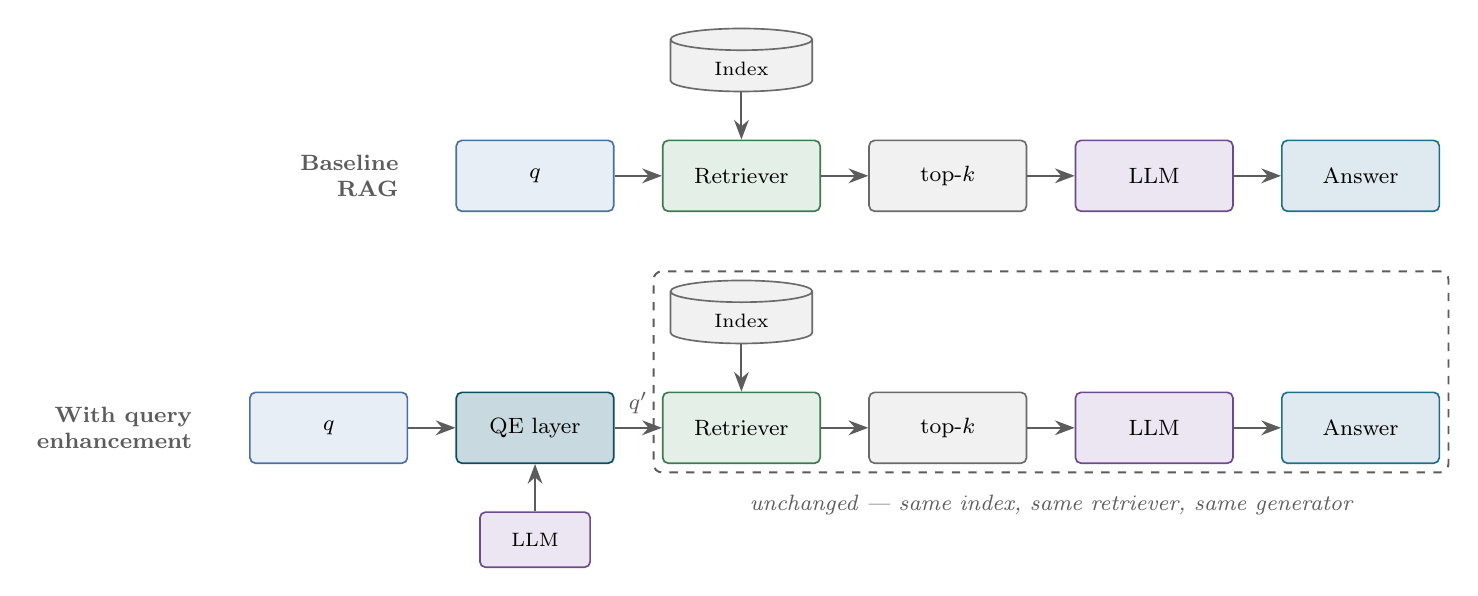
\begin{tikzpicture}[
    node distance=6mm and 6mm,
    box/.style={thBase, minimum width=20mm, minimum height=9mm, font=\footnotesize},
    rowlab/.style={font=\bfseries\footnotesize, color=thMuted, align=right}
]

  % ─── Row 2 (bottom): with query enhancement. Built first because it is longer. ──
  \node[thQuery, box]              (q2)  at (0,0)        {$q$};
  \node[thHi, box, right=of q2]    (qe)                  {QE layer};
  \node[thRet, box, right=of qe]   (r2)                  {Retriever};
  % Plain rectangle, not the thData cylinder: top-k is a set of retrieved passages,
  % not a store. Must match the row-1 node or the two rows stop being comparable.
  \node[thBase, box, right=of r2, draw=thDataS, fill=thDataF] (t2) {top-$k$};
  \node[thLLM, box, right=of t2]   (l2)                  {LLM};
  \node[thOut, box, right=of l2]   (a2)                  {Answer};

  \draw[thArrow] (q2) -- (qe);
  \draw[thArrow] (qe) -- (r2) node[thLabel, midway, above=0.5mm] {$q'$};
  \draw[thArrow] (r2) -- (t2);
  \draw[thArrow] (t2) -- (l2);
  \draw[thArrow] (l2) -- (a2);

  % generator that produces the expansion
  \node[thLLM, box, below=6mm of qe, minimum width=14mm, minimum height=7mm, font=\scriptsize] (gen) {LLM};
  \draw[thArrow] (gen) -- (qe);

  % ─── Row 1 (top): baseline. Retriever aligned with the row below. ──────────────
  \node[thRet, box]  (r1) at (r2 |- 0,32mm)  {Retriever};
  \node[thQuery, box, left=of r1]  (q1) {$q$};
  \node[thBase, box, right=of r1, draw=thDataS, fill=thDataF] (t1) {top-$k$};
  \node[thLLM, box, right=of t1]   (l1) {LLM};
  \node[thOut, box, right=of l1]   (a1) {Answer};

  \draw[thArrow] (q1) -- (r1);
  \draw[thArrow] (r1) -- (t1);
  \draw[thArrow] (t1) -- (l1);
  \draw[thArrow] (l1) -- (a1);

  % ─── Shared index, one per row ────────────────────────────────────────────────
  \node[thData, above=6mm of r1, minimum width=18mm, minimum height=8mm, font=\scriptsize] (i1) {Index};
  \draw[thArrow] (i1) -- (r1);
  \node[thData, above=6mm of r2, minimum width=18mm, minimum height=8mm, font=\scriptsize] (i2) {Index};
  \draw[thArrow] (i2) -- (r2);

  % ─── Row labels ───────────────────────────────────────────────────────────────
  \node[rowlab, left=6mm of q1] {Baseline\\RAG};
  \node[rowlab, left=6mm of q2] {With query\\enhancement};

  % ─── The modularity claim ─────────────────────────────────────────────────────
  \begin{scope}[on background layer]
    \node[draw=thMuted, dashed, rounded corners=3pt, line width=0.7pt,
          fit=(i2)(r2)(a2), inner sep=3pt] (unchanged) {};
  \end{scope}
  \node[thLabel, below=1.5mm of unchanged.south, anchor=north]
        {unchanged --- same index, same retriever, same generator};

\end{tikzpicture}
\end{document}
